Para o desenvolvimento desta monografia, faz-se necessário o entendimento de alguns conceitos, que foram abordados de maneira direta ou indireta no decorrer deste trabalho. Esses conceitos são apresentados nas subsseções seguintes.

\section{Arquitetura RISC}
\label{secao:arquiterura_risc}

A arquitetura RISC surgiu a partir da necessidade de se ter todos os componentes de um processador no mesmo chip - com a até então CISC não era possível. No entanto, para que isso ocorresse, algumas funcionalidades foram retiradas de dentro do processador, passando a complexidade para o software. Enquanto que as tarefas mais frequentes foram otimizadas e executadas diretamente pelo hardware, pois percebeu-se que a maior parte do trabalho era realizado por esse conjunto menor de instruções. Por exemplo, o suporte às linguagens de alto nível foi retirado dos circuitos integrados e passado para o software. O suporte ao microcódigo também foi retirado e as instruções são executadas em apenas uma microinstrução. Além da quantidade de instruções que foram reduzidas, o tamanho das mesmas foram encurtados e sempre que possível deveria demorar apenas um ciclo de relógio para serem executadas. O microcódigo deu lugar às pequenas (e em formato fixo) instruções em \textit{Assemly}, retirando, assim, o espaço da memória que era do microcódigo. Dessa forma, os compiladores passam a ter papel essencial para o bom funcionamento da arquitetura, pois estes tem toda a responsabilidade de otimizar os códigos durante o processo de compilação. \cite{silva:2008:comparacao}.

Com a redução do tamanho das instruções foi possível à implementação do \textit{pipelining} (que não é viável em ambientes com instruções de complexidade variável). Este recurso permite a execução de várias instruções paralelamente, o que reduz a quantidade média de ciclos por instrução (CPI ou \textit{Cycles Per Instruction}) e, consequentemente, o tempo de processamento dos programas (aumento de desempenho de processamento). Segundo \citet{silva:2008:comparacao}, outras duas características que permitiram a redução de ciclos/instrução, aumentando minimamente o tamanho do código na arquitetura RISC, são "a eliminação dos modos de endereçamento complexos e o aumento do número de registradores internos do processador". O aumento desses registradores tem a função de evitar a busca de variáveis locais na memória, pois estas são mantidas conforme a necessidade em bancos de registradores sempre que sub-rotinas são chamadas. \citet{azevedo:2014:comparacao} apresentam algumas características dessa arquitetura:

\begin{enumerate} 
	\item Registradores: 16-32.
	
	\item Tipos de dados: normalmente dois (inteiro e ponto flutuante).
	
	\item Instruções: \textit{Load/Store}, registradores gerais, operações sobre tipos de dados (\textit{datatypes}) nos registradores.
	
	\item Formato das instruções: tamanho fixo, dois tipos principais: \textit{Load/Store} ou R:=R op R.
	
	\item Codificação 1 instrução = 1 operando ou 1 operação.
	
	\item Objetivo do projeto: minimizar tempo de execução da instrução.
	
	\item Implementação: processador e software com alto grau de ligação, processador e \textit{cache} rápidos para instruções, instruções levam 1 ciclo de \textit{clock}, \textit{pipeline} simples.
	
	\item \textit{Caching}: essencial para as instruções.
	
	\item Filosofia: mover todas as funções para o software.
	
	\item Dispositivos: iPod, iPhone, iPad, Palm e PocketPC, Nintendo, Gameboy, Sun SPARC.
\end{enumerate}

\section{Arquitetura ARMv7 e ARMv8-A}
\label{secao:arquitetura_arm7_arm8}

O ARMv7\footnote{\textbf{ARM}: \textit{Advanced RISC Machine}.} possui arquitetura do tipo RISC de 32 \textit{bits}, \textit{pipeline} em três estágios e registradores \textit{load/store}. Isso faz com que o processador nunca fique ocioso, pois sempre estará executando diferentes estágios de instruções: buscando, decodificando e executando. Essa é uma maneira de se evitar conflitos entre estágios de outras arquiteturas. Outra característica é que o ARMv7 possui sete modos diferentes de execução que são usados para tratamento de exceções, de interrupções, entre outras funcionalidades. \cite[p.~16]{cruz:2013:desenvolvimento}. O Quadro \ref{quadro:modos_armv7} apresenta os sete modos e suas descrições.

\begin{quadro}[htb] \centering
	\begin{tabular}{lll}        \hline
		\textbf{Item}    & \textbf{Modo}           & \textbf{Descrição}                                             \\ \hline \hline
		1       & Usuário        & Execução normal de programas.                                   \\ 
		2       & Sistema        & Executa rotinas privilegiadas do sistema operacional.           \\ 
		3       & Supervisor     & Modo protegido para o sistema operacional.                      \\ 
		4       & IRQ            & Tratamento de interrupções comuns.                              \\ 
		5       & FIQ            & Tratamento de interrupções rápidas.                             \\ 
		6       & Abort          & Usado para implementar memória virtual ou proteção de memória.  \\ 
		7       & Indefinido     & Suporta emulação em software de co-processadores.      \\ \hline
	\end{tabular}
	\caption{Sete modos de execução do ARMv7: usuário, sistemas, supervisor, IRQ, FIQ, \textit{abort} e indefinido.}
	\ Fonte: \cite{cruz:2013:desenvolvimento}.
	\label{quadro:modos_armv7}
\end{quadro}

Todos esses modos apresentados no Quadro \ref{quadro:modos_armv7} também operam sob função especial (que pode ser ativada em tempo de execução) chamada de Thumb, onde o ARMv7 passa a ser um core de 16 \textit{bits} (o que aumenta o espaço da memória do programa). Esse processador possui dois conjuntos de instruções (16 e 32 \textit{bits}) sendo que o de 16 \textit{bits} é mais simples. Porém, todo o processamento é feito em 32 \textit{bits}, inclusive o acesso aos registradores. O ARMv7 possui melhor suporte às tradicionais operações de controle e às operações com ponto flutuante (se comparado com as famílias anteriores) principalmente devido às novas demandas de processamento gráfico (necessárias em jogos, processamento gráfico e outros). Há também a tecnologia NEON que melhora o DSP (\textit{Digital Signal Processor}), podendo chegar a 400\% de ganho no processamento digital de sinais. \cite[p.~17]{cruz:2013:desenvolvimento}.

A Figura \ref{figura:ref_001} apresenta a  arquitetura ARMv8-A que tem como base  a versão ARMv7 o que faz com que ela tenha todas as características apresentadas anteriormente. 

\begin{figure}[htb]  
	\centering
	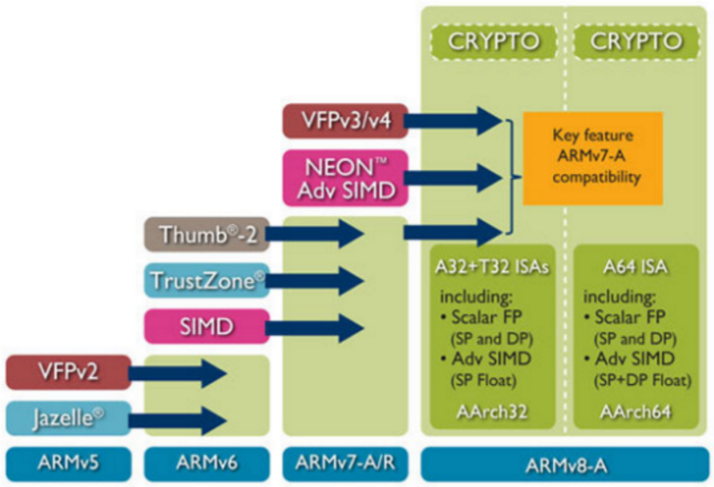
\includegraphics[width=.75\textwidth]{figuras/ref_001}
	\caption[Arquitetura ARM]{Arquitetura ARM: diferenças e semelhanças entre as arquiteturas ARMv5, ARMv6, ARMv7 e ARMv8-A, que mostra a compatibilidade das versões mais novas com as anteriores.} 
	\ Fonte: \cite{arm:2017:architecture}. 
	\label{figura:ref_001}
\end{figure}
A ARMv8-A tem sua arquitetura em 64 \textit{bits}, sendo compatível, portanto, com as versões 16 e 32 \textit{bits}. Além disso, a adição de instruções de 32 \textit{bits} permite, ainda, a otimização para requisitos emergentes. Um maior intervalo de endereçamento e instruções permitem a computação de novas categorias de aplicações para \textit{smartphones} e \textit{tablets}\footnote{\textbf{Texto original}: \textit{Increased availability of larger registers for general purpose and media instructions, a greater addressing range and cryptography instructions enable new categories of applications for superphone and tablet computing}.}. Outras características dessa arquitetura, descritas pela \citet{arm:2017:architecture}, que podem ser citadas, são:

\begin{enumerate}
	\item Registradores de uso geral de 64 \textit{bits}, SP (\textit{stack pointer}) e PC (\textit{program counter}).
	
	\item Processamento de dados de 64 \textit{bits} e endereçamento virtual estendido.
	
	\item Os estados de execução suportam três conjuntos de instruções principais:
	
	\begin{enumerate}
		\item AArch32: um conjunto de instruções de comprimento fixo de 32 \textit{bits}, aprimorado através das diferentes variantes de arquitetura;
		
		\item T32: (Thumb) introduzido como um conjunto de instruções de comprimento fixo de 16 \textit{bits}, posteriormente aprimorado para um conjunto de instruções de 16 e 32 \textit{bits} de comprimento misto na introdução da tecnologia Thumb-2;
		
		\item AArch64: é um conjunto de instruções de comprimento fixo de 64 \textit{bits} que oferece funcionalidade semelhante aos conjuntos de instruções ARM e Thumb.
	\end{enumerate}
	
\end{enumerate}

\section{Arquitetura x86}
\label{secao:arquitetura_x86}

Essa arquitetura teve seu nome (x86) originado do primeiro chip de 16 \textit{bits} da Intel, o 8086, que evoluiu para os modelos 80186, 80286, 80386 e 80486, todos com o sufixo "86",\ indicando a compatibilidade do conjunto de instruções com as versões anteriores. Inicialmente, essa arquitetura tinha seu conjunto de instruções do tipo CISC e, devido as necessidades do mercado, passou a utilizar instruções híbridas RISC/CISC. \cite{marmitt:2017:analise}. \citet{motyczka:2013:comparativo} explica que dessa forma "eles recebem instruções CISC, que são convertidas em instruções RISC para serem trabalhadas internamente buscando aperfeiçoar o processamento através do uso de \textit{pipeline}."\ São geradas micro operações parecidas com as instruções RISC, tendo-se assim uma máquina RISC dentro de uma x86. Mesmo sendo desenvolvido pela Intel, outras empresas passaram a utilizar a arquitetura x86 e, com o passar dos anos, esta se tornou padrão para computadores, notebooks e supercomputadores, sempre mantendo compatibilidades com as versões anteriores da arquitetura. A família x86 define um conjunto de tipos de instruções: movimentação de dados, aritmética e lógica, sequenciamento, manipulação de \textit{strings}, manipulação de \textit{bits}, suporte a linguagens de alto nível, entre outras.


\citet{mano:1993:computer} cita as principais características de processadores CISC:

\begin{enumerate}
	\item Número elevado de instruções (entre 100 e 250 instruções).
	
	\item Algumas instruções desempenham tarefas específicas e não são frequentemente utilizadas.
	
	\item Grande variedade de modos de endereçamento.
	
	\item Instruções com comprimento variável, assim utilizam diferentes números de \textit{bits} para codificar as instruções que dependem: quantidade de entradas da instrução, modos de endereçamento utilizados, entre outros fatores. \cite{lorenzoni:2012:analise}.
\end{enumerate}		


\section{Sistemas Embarcados}
\label{secao:sistemas_embarcados}

Os sistemas embarcados, também conhecidos como sistemas embutidos, são definidos como sistemas computacionais para uso específico ou dedicados. Estes estão se tornando cada vez mais populares e presentes na vida humana, principalmente por causa de algumas de suas vantagens, tais como: economia de energia, portabilidade, complexidade de processamento e baixo custo. A computação ubíqua - que diz respeito ao suporte computacional contínuo e permanente ao ser humano - tem como base os sistemas embarcados. Os núcleos de processamento de sistemas embarcados podem ser de propósito geral - que disponibilizam no hardware várias funções já implementadas, executam as mais variadas aplicações e funcionam com a execução de um programa - na qual tarefas como buscar, decodificar e executar instruções afetam diretamente o desempenho; ou podem ser de uso específico, possuindo circuitos integrados que são desenvolvidos para um conjunto específico de funções (ASIC - \textit{Aplication Specific Integrated Circuit}). \cite{cruz:2013:desenvolvimento}.

Os projetos de sistemas embarcados podem apresentar uma grande flexibilidade não apenas do ponto de vista da programação (software), mas também em relação à parte física (hardware), especialmente quando implementados em sistemas reconfiguráveis. Hardware específico ou dedicado, normalmente, é separado para tarefas que exigem alto poder de processamento, assim as demais funcionalidades são implementadas por meio de software \cite{wei:2008:research}.
Essa característica faz com que os sistemas de uso específico apresentem um desempenho melhor (na execução de tarefas) do que os sistemas de propósito geral.

\section{Raspberry Pi}
\label{secao:raspberry_pi}

É um pequeno computador que possui memória primária e secundária, CPU (unidade central de processamento), GPU (unidade de processamento gráfico), sistema operacional (SO), conectores USB (\textit{Universal Serial Bus}), saída de vídeo, saída de áudio, interface \textit{Ethernet}, entre outros. Possui baixo custo e possibilidade de aplicação em problemas reais. Possui, ainda, pinos (GPIO – \textit{General Purpose Input/Output}) que possibilitam o recebimento e o envio de sinais elétricos. \cite[p.~3]{sheid:2015:raspberry}. 
\citet[p.~19]{coutinho:2016:sistema} afirma que “desenvolvida pela fundação Raspberry Pi, no Reino Unido, a plataforma Raspberry é um computador de baixo custo, pequeno, \textit{Open Source} e com interfaces para vários periféricos.” A \citet{fundacaoraspberry:2017:raspberry} define esta placa como "um pequeno computador capaz de ser usado em projetos eletrônicos, e para muitas das coisas que seu PC de mesa faz, como planilhas, processamento de texto, navegar na internet e jogar. Ele também reproduz vídeo de alta definição." Suas principais características são:

\begin{enumerate}
	\item 1.2GHz 64-\textit{bits quad-core} ARMv8-A CPU com memória \textit{cache} de 32kB nível 1 e 512kB nível 2.
		
	\item 1GB RAM LPDDR2 (900 MHz).
		
	\item 4 portas USB 2.0.
		
	\item 40 pinos GPIO.
		
	\item Porta \textit{Full} HDMI.
		
	\item Porta 10/100 \textit{Ethernet}.
		
	\item \textit{Combined} 3.5mm \textit{audio jack and composite video}.
		
	\item Interface de câmera (CSI).	
	
	\item \textit{Display} interface (DSI).
		
	\item Slot para cartão Micro SD (agora \textit{push-pull}, em vez de \textit{push-push}).
		
	\item VideoCore IV (Núcleo gráfico 3D) - suporte a OpenGL ES 2.0, acelerador de hardware OpenVG, alta capacidade de codificação e decodificação em perfil 1080p30 H.264. A GPU tem capacidade de 1Gpixel/s, 1.5Gtexel/s ou 24GFLOPs em processamento de propósito geral e apresenta várias filtragens de texturas,  além de infra-estrutura DMA (\textit{Direct Memory Access})\footnote{\textbf{Texto original}: \textit{VideoCore IV 3D graphics core - The GPU provides OpenGL ES 2.0, hardware-accelerated OpenVG, and 1080p30 H.264 high-profile encode and decode. The GPU is capable of 1Gpixel/s, 1.5Gtexel/s or 24 GFLOPs of general purpose compute and features a bunch of texture filtering and DMA infrastructure}.}.
	 	
	\item Completa compatibilidade com os Raspberry Pi 1 e 2. A Figura \ref{figura:ref_002} apresenta a distribuição dos componentes na placa e a Tabela \ref{tabela:consumo_raspberry} apresenta os dados necessários para a alimentação da placa. Os pinos GPIO podem fornecer até 50mA com segurança (note que isso significa que 50mA distribuídos em todos os pinos: um pino individual GPIO só pode seguramente fornecer até 16mA).
\end{enumerate}	

\begin{figure}[htb]  
	\centering
	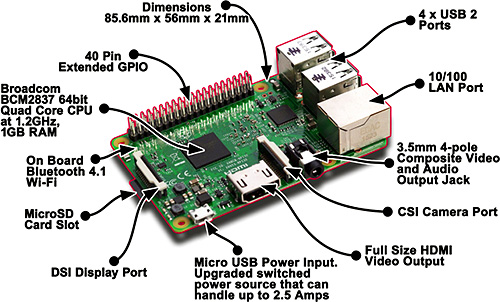
\includegraphics[width=.8\textwidth]{figuras/ref_002}
	\caption[Raspberry Pi 3 Modelo B]{Componentes da Raspberry Pi 3 Modelo B, sendo estes de entrada e saída (gpio, ethernet, USB, HDMI, interface CSI e DCI, conector áudio, conector fonte de energia, slot SD card), bluetooh 4.1 e Wi-Fi.}
	\ Fonte: \cite{fundacaoraspberry:2017:raspberry}.
	\label{figura:ref_002}
\end{figure}

\begin{table}[htb] \centering
	\caption{Modelos e características da raspberry, sendo capacidade recomendada de alimentação, corrente máxima consumida pelos periféricos USB e o consumo de corrente ativa típico na placa.} \label{tabela:consumo_raspberry}
	\begin{tabular}{c|ccc}        \hline
		& \textbf{Capacidade}  & \textbf{Corrente máxima} &   \textbf{Consumo de}    \\ 
		\textbf{Raspberry Pi} &   \textbf{recomendada da}    & \textbf{consumida pelos} & \textbf{corrente ativa}  \\
		& \textbf{fonte de alimentação} & \textbf{periféricos USB} & \textbf{típico na placa} \\ \hline \hline          
		Model A 	 &        700mA         &     500mA       &      200mA      \\ 
		Model B	 	 &	      1,2A          &      500mA      &      500mA      \\ 
		Model A+ 	 &        700mA         &      500mA      &      180mA      \\ 
		Model B+ 	 &        1,8A          &   600mA/1,2A    &      330mA      \\  
		&                      &(\textit{switchble}) &             \\ 
		2 Model B	 & 	      1,8A          &   600mA/1,2A    &        -        \\  
		&                      &(\textit{switchble}) &             \\ 
		3 Model B	 &  	  2,5A          &      1,2A       &      ~400mA     \\ 
		Zero W		 &   	  1,2A          &\textit{Limited by} &      150mA   \\ 
		&                      &\textit{PSU only} &                \\
		Zero		 &        1,2A          &\textit{Limited by}&      100mA    \\ 
		&                      &\textit{PSU only} &                \\ \hline
	\end{tabular}
	\\ Fonte: \cite{fundacaoraspberry:2017:raspberry}.
\end{table}

\citet[p.~20]{coutinho:2016:sistema} afirma  que “existem várias versões diferentes de sistemas operacionais (SOs) compatíveis com a plataforma, sendo que o SO do Raspberry é instalado no cartão SD do dispositivo.” Para fins de uso não específico da placa, é recomendado a utilização da distribuição Linux Raspbian, recomendação esta feita pela fabricante que ainda acrescenta: “Raspbian é um sistema operacional livre baseado no Debian, otimizado para o hardware Raspberry Pi. Raspbian vem com mais de 35.000 pacotes: software pré-compilado empacotado em um formato agradável para fácil instalação em seu Raspberry Pi.” \cite{fundacaoraspberry:2017:raspberry}.  

\section{Algoritmo Genético}
\label{secao:AG}

Os Algoritmos Genéticos (AGs) são uma técnica de Inteligência Artificial baseada no princício da seleção e evolução natural de orgamimos biológicos (Darwinismo) em que os indivíduos que mais se adaptarem ao ambiente terão mais chance de sobreviver e se reproduzirem. Os AGs são amplamente aplicados em busca e otimização de resultados (buscam a melhor solução para um determinado problema). (\cite{pacheco:1999:algoritmos}. \cite{silva:2001:otimizacao}). 

Um AG trabalha de forma aleatória mas orientada para algumas regras probabilísticas, de acordo com os mecanismos de reprodução e genética natural. Primeiro, cria-se uma população inicial (em que cada indivíduo é uma solução para o problema). Esta população é então avaliada para se conhecer quais são os melhores indivíduos (com melhor \textit{fitness} ou melhor aptidão). Estes devem ter maiores chances de cruzamento para que se garanta a reprodução e propagação do material genético para as proximas gerações. Algumas estratégias sugerem passar os melhores indivíduos direto para o proxima geração. Os indivíduos são implementados de forma que as características possam ser trocadas com outros indivíduos, tendo-se, assim, a reprodução. Cruzando-se os indivíduos, gera-se uma nova população que deve ser do mesmo tamanho da população inicial, a população antiga é substituida, então, por esta nova. De forma percentual e aleatória, aplica-se a mutação sobre a população (alteração dos cromossomos pode gerar indivíduos melhores). Esses procedimentos são repeditos até que se tenha uma solução aceitável ou até que se atinja um número máximo de gerações. A Figura \ref{figura:ref_007} mostra um fluxograma básico e o Algoritmo \ref{algoritmo:ag} apresenta o pseudocódigo básico de um AG. (\cite{holland:1992:adaptation} e \cite{goldberg:1989:genetic} apud \cite{avila:2002:algoritmos}).

\begin{figure}[htb]  	
	\centering	
	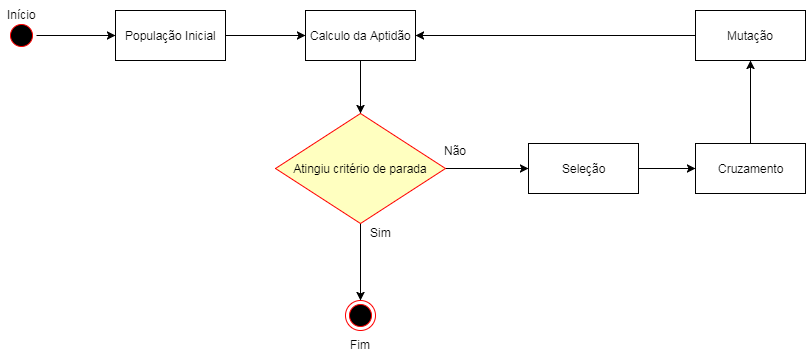
\includegraphics[width=\textwidth]{figuras/ref_007}
	\caption[Fluxograma de um AG]{Fluxograma de um AG básico, que gera população inicial aleatoriamente, avalia esta população, verifica o critério de parada, faz a seleção dos melhores indivíduos, realiza o cruzamento (o que gera nova população), realiza a mutação e volta ao critério de parada. Caso não tenha sido atingido, o algoritmo volta ao passo de seleção e, assim continua até que se satisfaça o critério de parada.} 	
	\label{figura:ref_007}
\end{figure}

\begin{algoritmo}[!htb]
	\begin{algorithmic}[1]
		\\$gerac \leftarrow 0$;    //inicializa contador gerações
		\\$Pop(gerac) \leftarrow Inicializa\_populacao()$;    //população inicial gerada aleatoriamente
		\State$Avalia(Pop(gerac))$;    //avalia população inicial
		\Repeat 
			\State$ P \leftarrow Seleciona(Pop(gerac)) $;    //seleciona indivíduos para cruzamento
			\State$ P \leftarrow cruzamento(P) $;    //cruzamento ou recombinação dos indivíduos
			\State$ P \leftarrow mutacao(P) $;    //operação de mutação nos indivíduos
			\State$ gerac \leftarrow gerac + 1 $;    //incrementação do contador de gerações
			\State$ Pop(gerac) \leftarrow atualiza(P)$; //atualiza a população atual
			\State$ Avalia(Pop(gerac))$; // avalia população atual
		\Until      //satisfaça condição de parada
		\\Print(Avalia(Pop(gerac)));
	\end{algorithmic}
	\caption{Pseudocódigo do AG clássico} \label{algoritmo:ag}
\end{algoritmo}

Os indivíduos devem possuir cromossomos, sendo que estes devem ter genes que são caracterésticas ou informações sobre os indivíduos. Em outras palavras é o material genético do indivíduo que será trocado com outros indivíduos durante o cruzamento. Sendo assim, faz-se necessário uma função que seja capaz de avaliar o \textit{fitness} dos indivíduos. A codificação do indivíduo e da função de avaliação tem grande importância, pois possui a responsabilidade de relacionar o algoritmo com o problema real, avaliando quão boas são as características dos indivíduos em relação ao problema. \cite{neto:2011:computaccao}.

\section{O Problema do Caixeiro Viajante}
\label{secao:caixeiro_viajante}

O Problema do Caixeiro Viajante (PCV, do inglês: \textit{Traveling Salesman Problem} - TSP) é um dos mais conhecidos problemas de otimização combinatória. Basicamente, consiste no problema de encontrar a melhor rota possível (que pode ser menor caminho, caminho de menor custo, entre outros) em um conjunto de cidades, sendo que cada cidade só pode ser visitada uma única vez no trajeto. Quando o percurso entre duas cidades (ou nós) x e y não sofre interferência do sentido (Pxy = Pyx), o PCV é chamado de simétrico; quando há diferença em virtude do sentido do trajeto, é chamdo de PCV assimétrico. O simétrico é, em geral, mais difícil de ser resolvido que o assimétrico. O PCV "tem sido usado como \textit{benchmark} para avaliação de novos algoritmos e estratégias de solução que envolvem busca tabu, algoritmos genéticos, \textit{simulated annealing}, redes neurais artificiais, entre outras." \cite{cunha:2002:experimentos}. O estudo e aplicação do PCV não se restringe ao cenário de desempenho computacional, mas está presente em inúmeras áreas (pesquisa operacional, matemática, física, biologia, inteligência artificial, entre outros) em vários tipos de problemas reais, como por exemplo, roteirização de veículos e \textit{design} de circuitos.

\begin{citacao}
	Sob a ótica de otimização, o PCV pertence à categoria conhecida como NP-difícil (do inglês NP-\textit{hard}), o que significa que possui ordem de complexidade exponencial. Em outras palavras, o esforço computacional para a sua resolução cresce exponencialmente com o tamanho do problema (dado pelo número de pontos a serem atendidos). \cite{cunha:2002:experimentos}.
\end{citacao}

Problemas dessa categoria não podem ser resolvidos de maneira ótima em tempo viável, assim as técnicas atuais para resolução são conhecidas como heurísticas, pois não garantem um resultado ótimo, mas sim um resultado aproximado. Segundo \citet{helsgaun:2000:effective}, as heurísticas para resolução do PCV podem ser implementadas de duas formas:

\begin{enumerate}
	\item Métodos de contrução de roteiros: os nós ou cidades são inseridos no roteiro de forma gradual e sequencial, sem que a solução parcial seja avaliada e/ou melhorada, assim a sequencia é montada e não é alterada mais.  
	
	\item Métodos de melhorias de roteiros: através de um roteiro já obtido, com alguma técnica, busca-se melhorar o roteiro (diminuir o custo ou a distância do trajeto, por exemplo). Há autores que consideram uma terceira forma, que une a técnica de construção e a de melhoria de trajeto. \cite{cunha:2002:experimentos}.
\end{enumerate}

Segundo \citet{laporte:2000:classical} e \citet{reinelt:1994:traveling}, a construção de roteiros pode ser dada através:

\begin{enumerate}
	\item método do vizinho mais próximo;	
	\item método da inserção;	
	\item método das economias;	
	\item heurísticas baseadas em árvores de cobertura (\textit{spanning trees}). \cite{cunha:2002:experimentos}.
\end{enumerate}

\section{Sistemas Paralelos}
\label{secao:sistemas_paralelos}

Sistema paralelos são do tipo MIMD (\textit{Multiple Instruction, Multiple Data}), pois possuem múltiplos fluxos de instruções e múltiplos fluxos de controle, como os processadores \textit{multicore}, os computadores com múltiplos processadores e os \textit{clusters}. O termo \textit{multicore} é usado para definir sistemas com vários núcleos em um único chip e também sistemas com núcleos em chips separados ou independentes. Nos sistemas com mais de um núcleo que compartilham memória, o gerenciamento e sincronismo da mesma torna-se ainda mais rigoroso para evitar inconsistências nos dados. Para que os recursos implementados por sistemas paralelos sejam realmente utilizados, os softwares que são executados nos mesmos devem ter suporte para essas arquiteturas. Para isso, os algoritmos devem ter três características básicas: distribuição das tarefas para os diferentes processadores (mapeamento), execução compartilhada das tarefas conforme a dependência de dados (compartilhamento) e identificação dos dados que trafegam entre os processadores (identificação). \cite{lima:2016:implantacao}. 

\citet{hwang:1987:advanced} sugere que há diferentes níveis de paralelismo, sendo estes:

\begin{enumerate}	
	\item Nível 5: processos (\textit{jobs}) e programas independentes;
	\item Nível 4: sub-processos e pontes de programas;
	\item Nível 3: rotinas, sub rotinas e co-rotinas;
	\item Nível 2: iterações (\textit{loosp});
	\item Nível 1: instruções (\textit{pipeline}). \citet{navaux:1989:introducao}.
\end{enumerate}

O nível mais alto é o algorítmico e o inferior (de instruções) é implementado em hardware - quanto mais baixo o nível mais fina é a granularidade do processamento. O paralelismo explora um ou a combinação desses níveis e a tendência é de que quanto mais destes níveis implementados na mesma máquina, mais poderosa esta será. Alguns autores sugerem que há também:

\begin{enumerate}
\item Paralelismo em nível de \textit{bit} (\textit{bits} de uma instrução são processados em paralelo).
	
\item Paralelismo em nível de dados (dados são acessados em paralelo e seus resultados são combinados).

\item Paralelismo em nível de tarefas (fluxos de controle independentes para cada tarefa).
\end{enumerate}

\section{Biblioteca OpenMP}
\label{secao:openmp}

É uma biblioteca desenvolvida para processamento paralelo de algotimos utilizando memória compartilhada, em que através de diretivas de compilação, rotinas da biblioteca e variáveis de ambiente tem-se a paralelização do algoritmo de forma que o código sequencial é minimamente modificado e, por ser de memória compartilhada, as \textit{threads} comunicam-se através de variáveis compartilhadas. \cite{rodrigues:2012:proposta}.

O uso desse tipo de variável exige um controle de acesso rigoroso para evitar problemas com inconsistência nos dados ou resultados errôneos. Há a implementação de uma política de acesso para que, enquanto uma \textit{thread} realizar a escrita, nenhuma outra possa ler ou escrever na variável em questão - fazendo com que as demais que necessitem acessar entrem em estado de espera (este problema é conhecido como \textit{race condition} ou condição de corrida). Já o processo de leitura pode ser feito simultaneamente por todas as \textit{threads} do perocesso. \cite{openmp:2011:application}. 

Contudo, quanto menor for o uso de variaveis compartilhadas e menor for a dependência entre as \textit{threads}, melhor será o desempenho do algoritmo. Dessa forma, diminui-se gargalos causados por acessos ou pela espera dos acessos a estas variáveis. \cite{rodrigues:2012:proposta}.